\section{Druhá verze}


Druhá verze trezoru už byla vybavená signalizačním kruhem o dvanácti LED kolem uprostřed dveří
umístěného enkodéru. Jako základ trezoru jsem použil první mechanický trezor, %todo odkaz
 ze kterého jsem odstranil zamykací kola 
a doplnil jej o servo, řídící elektroniku a již zmíněný kruh LED a~enkodér.
%Vzhledem k tomu, že se jednalo jen o hrubý prototyp, neměl specializovanou desku~a elektroniku  tedy tvořila jen změť kabelů 
% a kousek univerzální desky, takže nemám elektronickou variantu tohoto zapojení. % [schéma jsem kreslil jen na tabuli a to asi rok 
% zpátky, takže když bych došel k závěru že je potřeba, tak se dá udělat, ale je to práce navíc a nepovažoval bych to za podstatné]

Trezor měl pro komunikaci s uživatelem tedy kruh o dvanácti LED a~jeden vstupní prvek -- enkodér s tlačítkem.
Ovládání bylo od výbavy trezoru odvozené a trezor se zmáčknutím tlačítka na enkodéru zapnul a tlačítko pak dál sloužilo jako potvrzování výběru.
Uživatel tak mohl pomocí enkodéru vybírat jedinou rozsvícenou ledku a stiskem potvrdit. 

Vstupní kód tedy mohl vypadat 
například jako čas a uživatel ho zadal na kruhu odvozeném od ručičkových hodin, proto právě dvanáct LED.
Konkrétní ovládání je pochopitelně závislé na nahraném programu a mohlo by se tedy jednoduše změnit do libovolné podoby --
to, co popisuji, je jen konkrétní možnost, kterou jsem použil.

\begin{figure}[htbp]
    \centering
    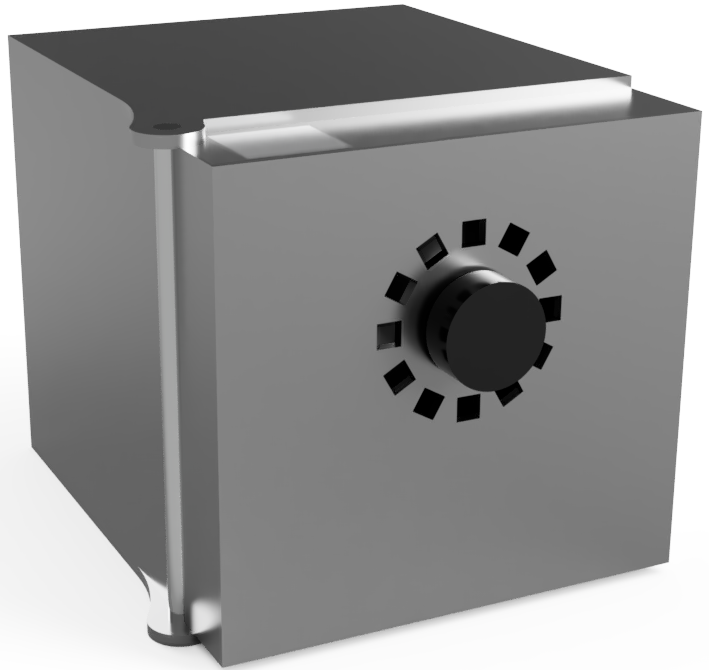
\includegraphics[width=\textwidth]{kapitoly/obrazky/E2/predni_render.png}
    \caption{Render varianty E2}
    \label{fig:E2-render}
\end{figure}

\newpage